\section{Grupo de Processo Planejamento}

\begin{frame}
 \frametitle{GRUPO DE PROCESSOS (“FASE”) – PLANEJAMENTO}
  \begin{figure}
   \centering
   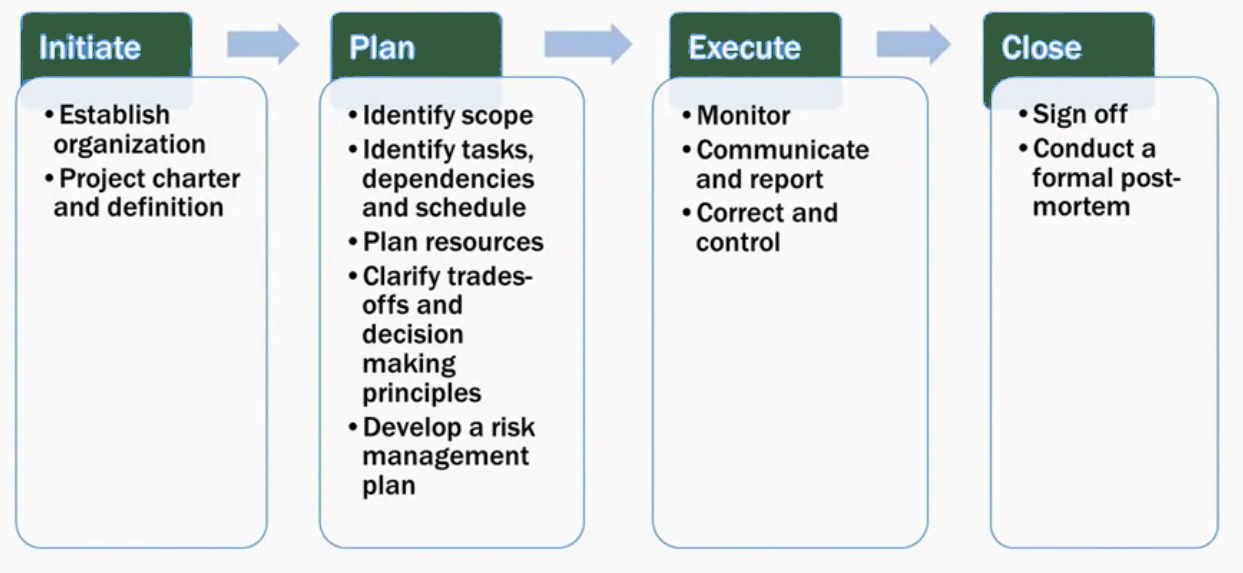
\includegraphics[width = 0.9\textwidth]{figs/fig0.png}
  \end{figure}
\end{frame}

\begin{frame}
 \frametitle{Grupo de Processos de planejamento}
 \begin{block}{Definição PMBok}
  O grupo de processos de planejamento consiste dos \textbf{processos} realizados para estabelecer o \textbf{escopo}
total do esforço, definir e refinar os \textbf{objetivos} e desenvolver o  \textbf{curso de ação necessário} para alcançar esses
objetivos.
 \end{block}
\end{frame}

\begin{frame}
 \frametitle{Grupo de Processos de planejamento}
 \begin{block}{Definição PMBok}
O \textbf{benefício principal} deste grupo de
processos é \textbf{delinear a estratégia e a tática}, e também o \textbf{curso de ação} ou o caminho para a conclusão do
projeto ou da fase com sucesso.
\end{block}
\end{frame}

\begin{frame}
 \frametitle{GRUPO DE PROCESSOS (“FASE”) – PLANEJAMENTO}
  \begin{figure}
   \centering
   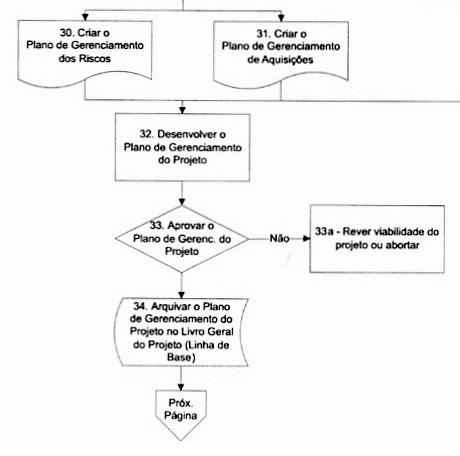
\includegraphics[height = .9\textheight]{figs/fig17.png}
   \caption{Fluxograma}
  \end{figure}
\end{frame}

\begin{frame}
 \frametitle{Fontes de Incertezas}
  \begin{figure}
   \centering
   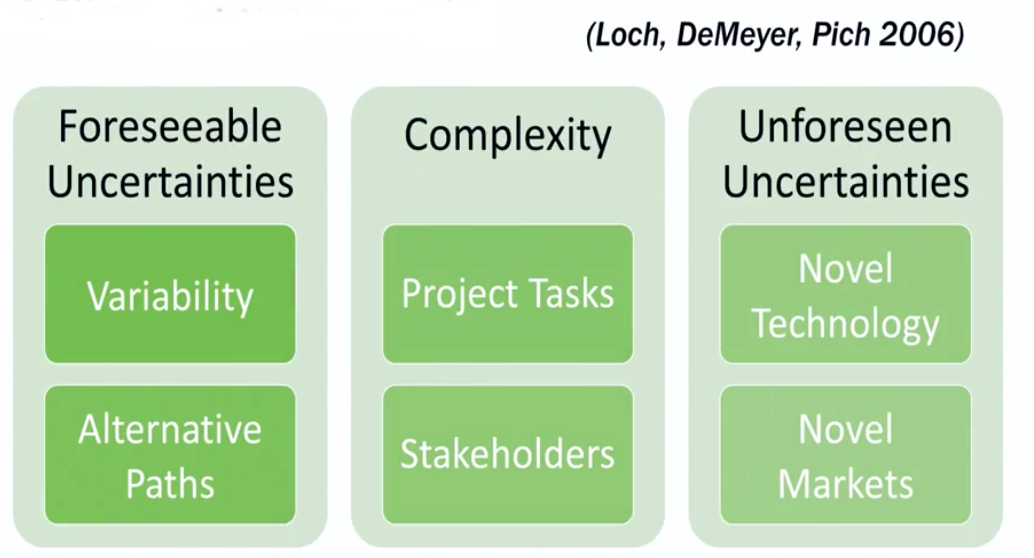
\includegraphics[width = 0.9\textwidth]{figs/fig1.png}
  \end{figure}
\end{frame}


\begin{frame}
 \frametitle{Fontes de Incertezas}
  \begin{figure}
   \centering
   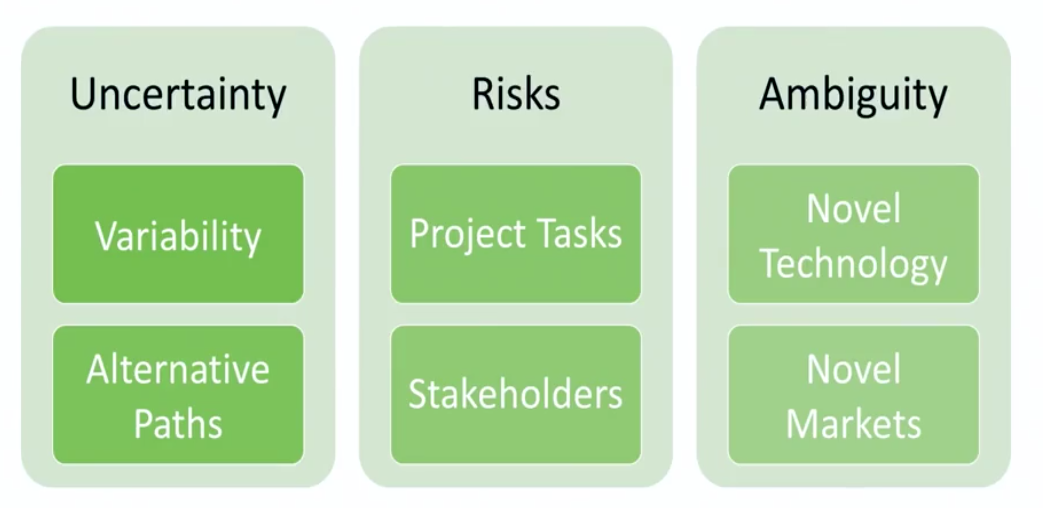
\includegraphics[width = 0.9\textwidth]{figs/fig2.png}
  \end{figure}
\end{frame}

\begin{frame}
 \frametitle{Demanda e incertezas tecnológicas da indústria}
  \begin{figure}
   \centering
   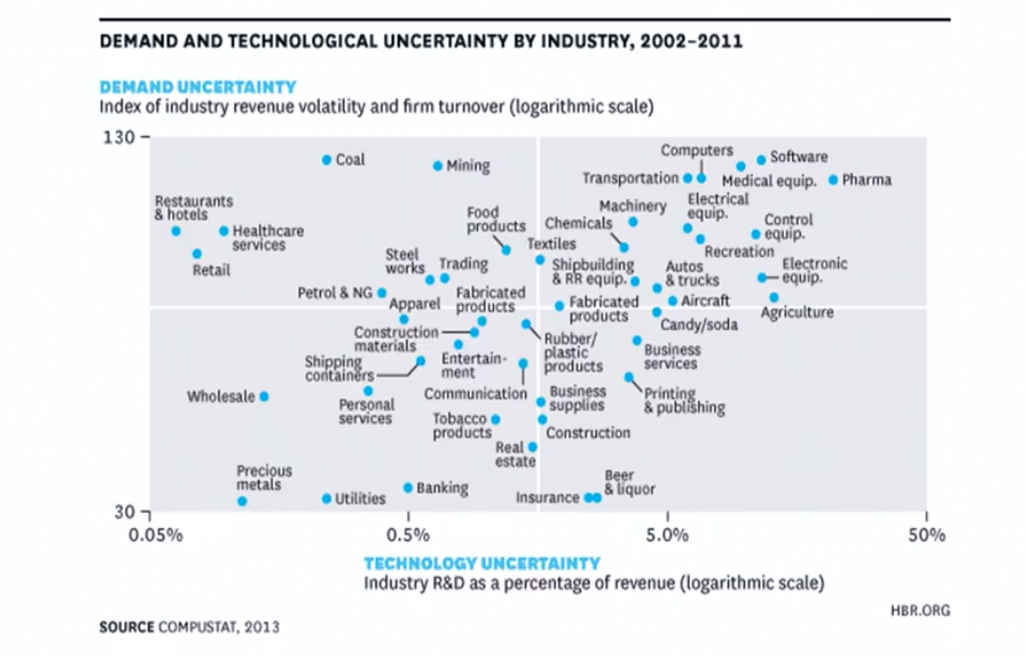
\includegraphics[width = 0.9\textwidth]{figs/fig3.png}
  \end{figure}
\end{frame}


\begin{frame}
 \frametitle{Adequação do planejamento para o tipo de risco}
  \begin{figure}
   \centering
   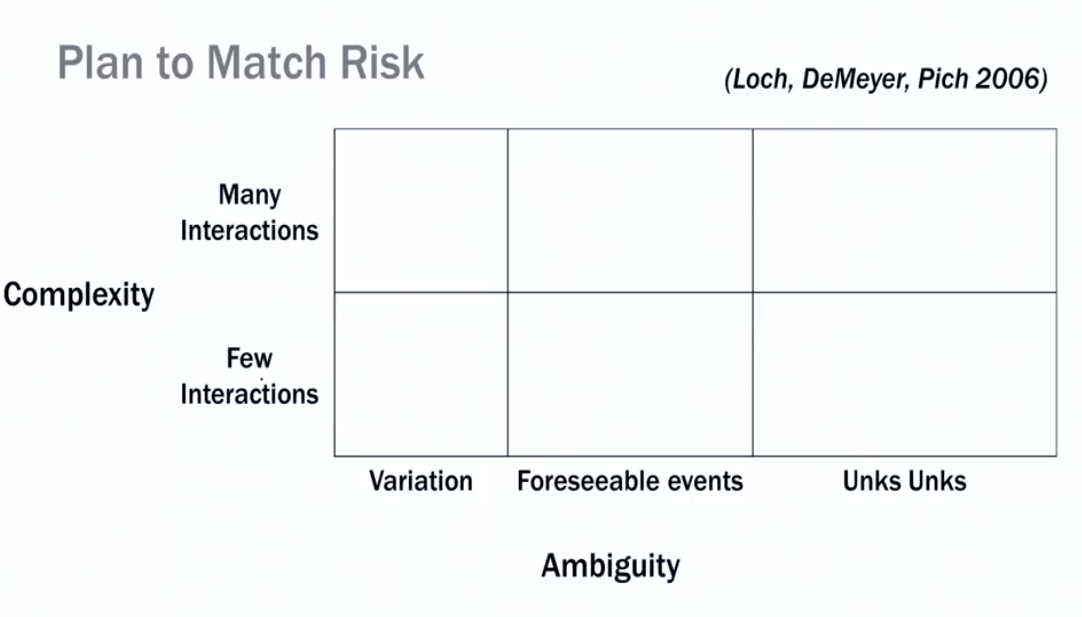
\includegraphics[width = 0.9\textwidth]{figs/fig4.png}
  \end{figure}
\end{frame}

\begin{frame}
 \frametitle{Adequação do planejamento para o tipo de risco}
  \begin{figure}
   \centering
   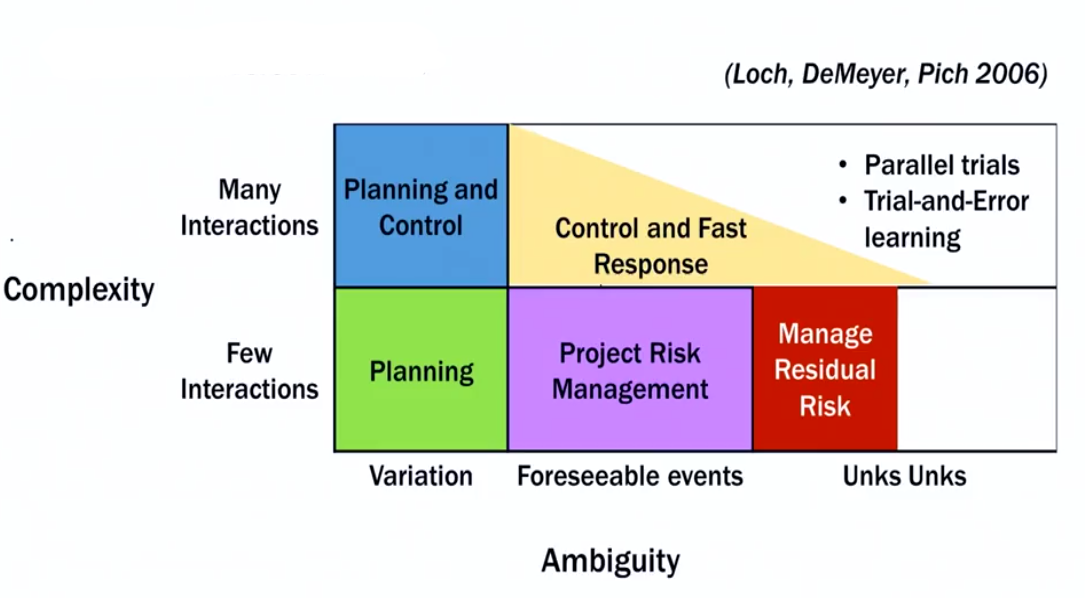
\includegraphics[width = 0.9\textwidth]{figs/fig5.png}
  \end{figure}
\end{frame}

\begin{frame}
 \frametitle{Gestão de riscos em projetos}
  \begin{figure}
   \centering
   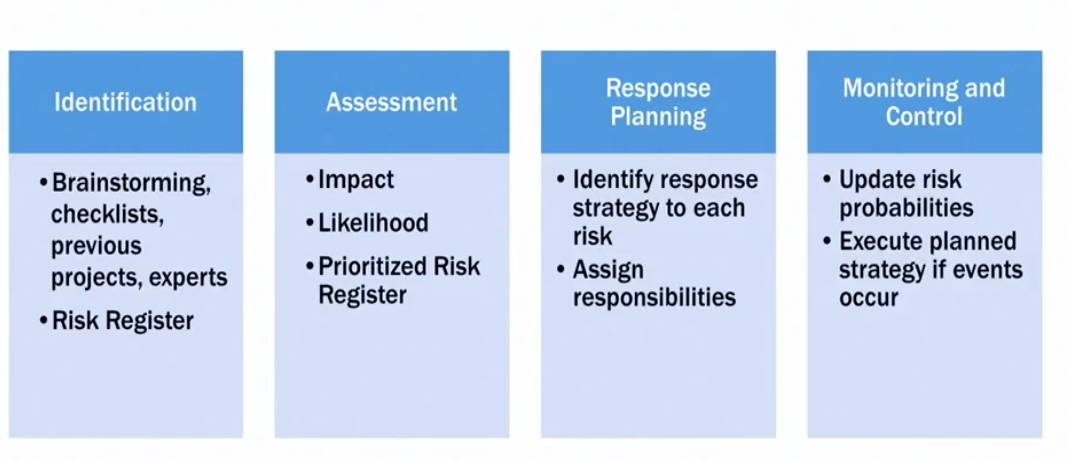
\includegraphics[width = 0.9\textwidth]{figs/fig6.png}
  \end{figure}
\end{frame}

\begin{frame}
 \frametitle{Avaliação do Risco}
  \begin{figure}
   \centering
   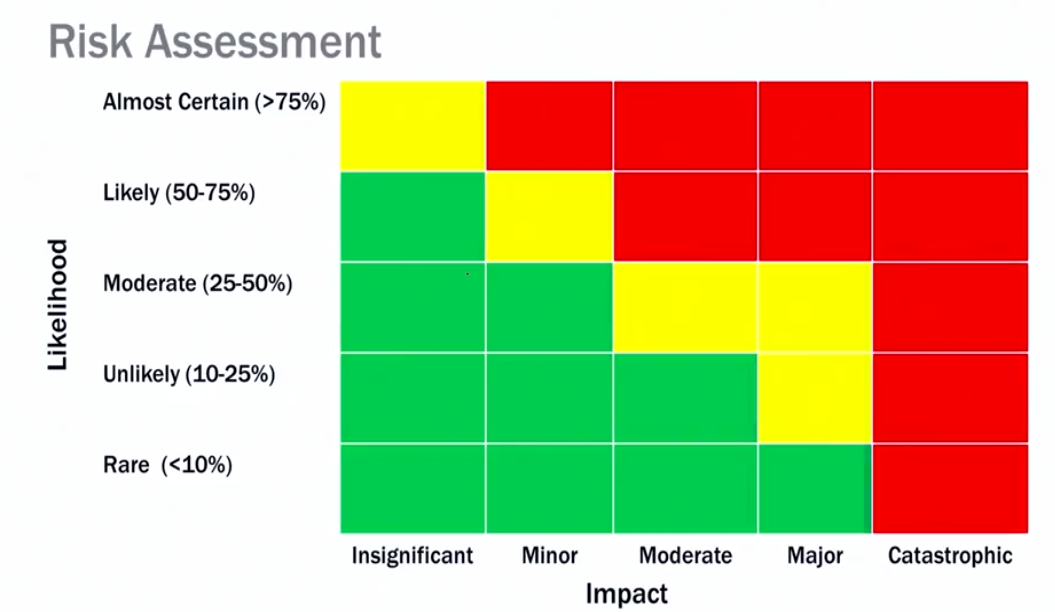
\includegraphics[width = 0.9\textwidth]{figs/fig7.png}
  \end{figure}
\end{frame}

\begin{frame}
 \frametitle{Avaliação do Risco}
  \begin{figure}
   \centering	
   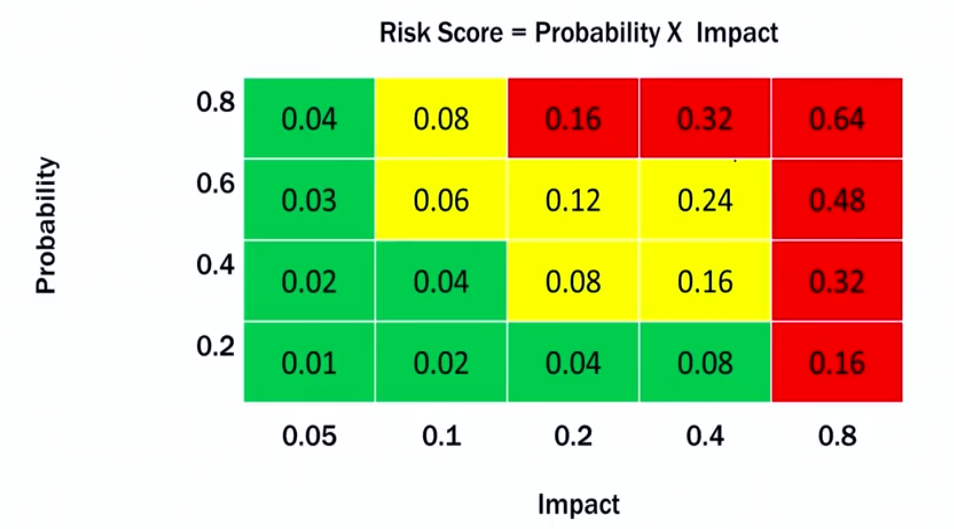
\includegraphics[width = 0.9\textwidth]{figs/fig8.png}
  \end{figure}
\end{frame}

\begin{frame}
 \frametitle{Registro de Riscos}
  \begin{figure}
   \centering
   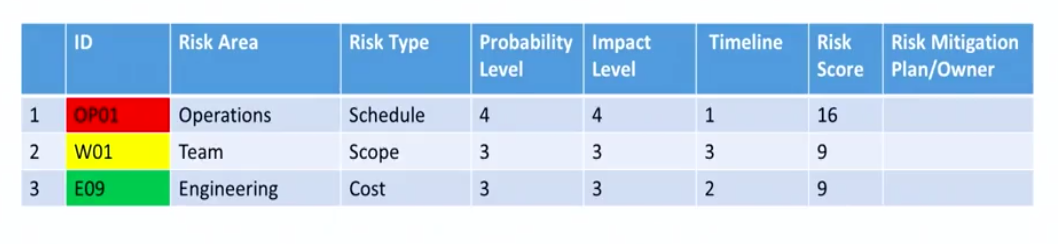
\includegraphics[width = 0.9\textwidth]{figs/fig9.png}
  \end{figure}
\end{frame}

\begin{frame}
 \frametitle{Exemplo - Projeto Start up}
  \begin{figure}
   \centering
   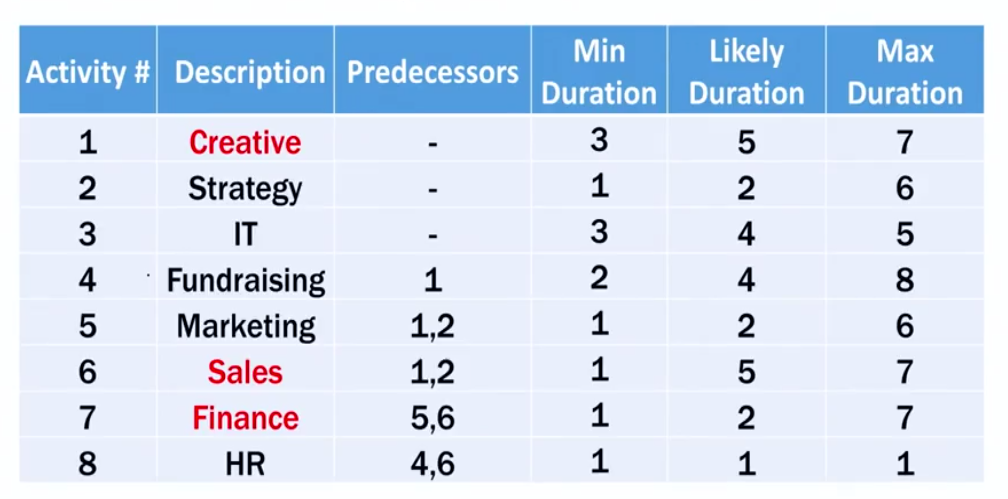
\includegraphics[width = 0.9\textwidth]{figs/fig10.png}
  \end{figure}
\end{frame}

\begin{frame}
 \frametitle{tornado chart}
  \begin{figure}
   \centering
   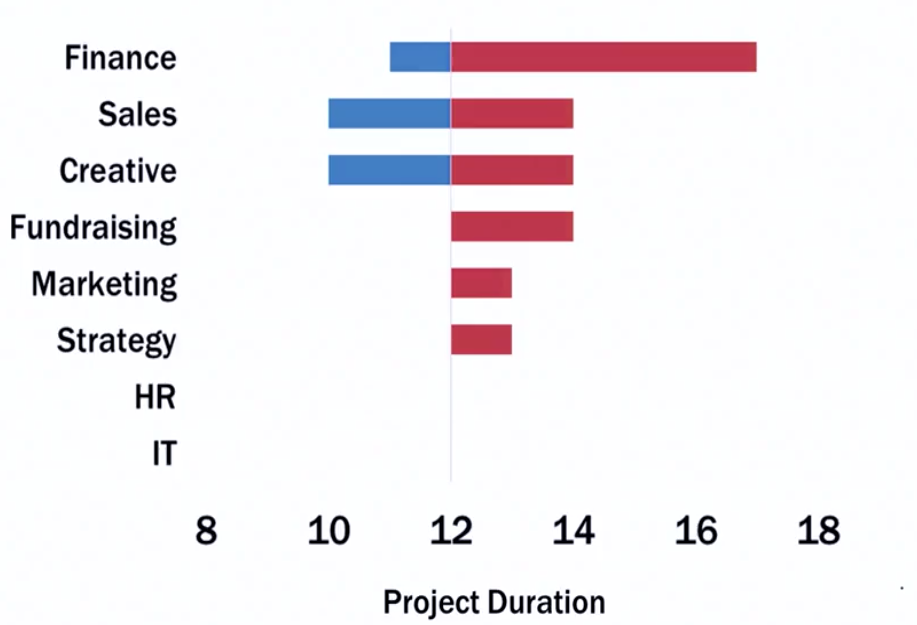
\includegraphics[width = 0.9\textwidth]{figs/fig11.png}
  \end{figure}
\end{frame}

\begin{frame}
 \frametitle{Análise de Risco}
  \begin{figure}
   \centering
   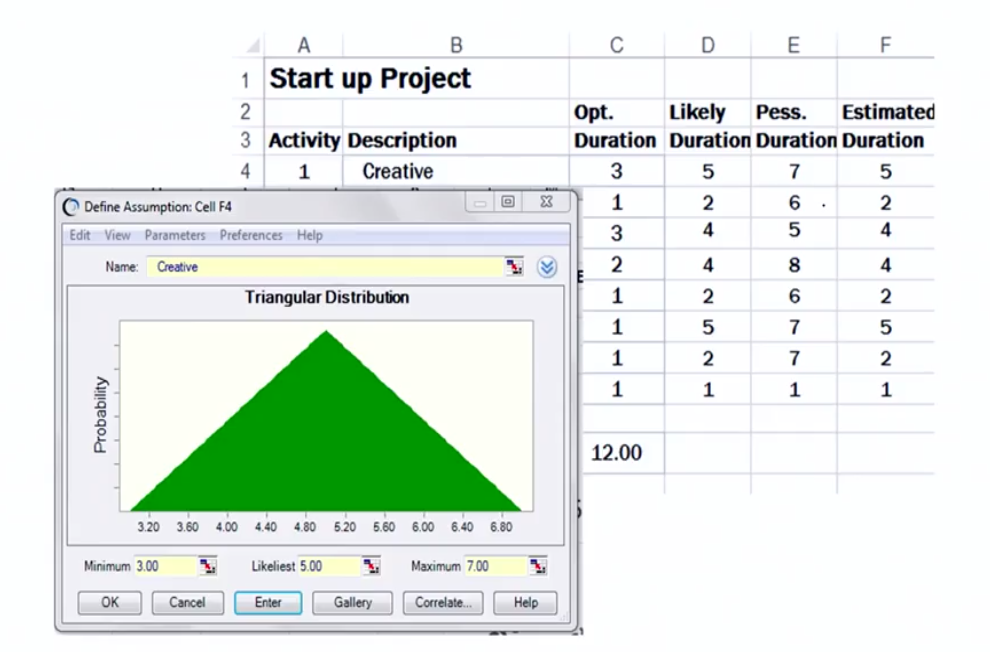
\includegraphics[width = 0.9\textwidth]{figs/fig12.png}
  \end{figure}
\end{frame}

\begin{frame}
 \frametitle{Análise de Risco}
  \begin{figure}
   \centering
   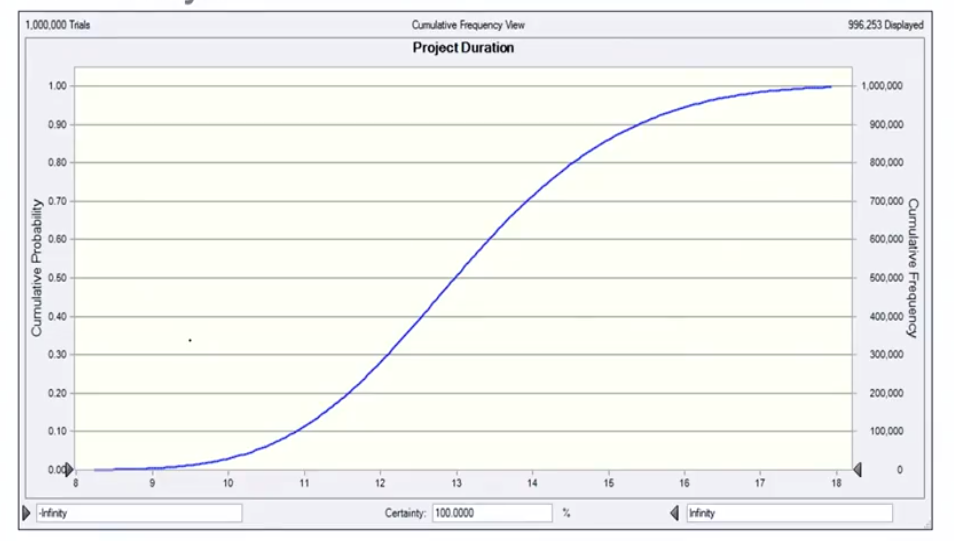
\includegraphics[width = 0.9\textwidth]{figs/fig13.png}
  \end{figure}
\end{frame}

\begin{frame}
 \frametitle{Roadmap no lugar de plano}
  \begin{figure}
   \centering
   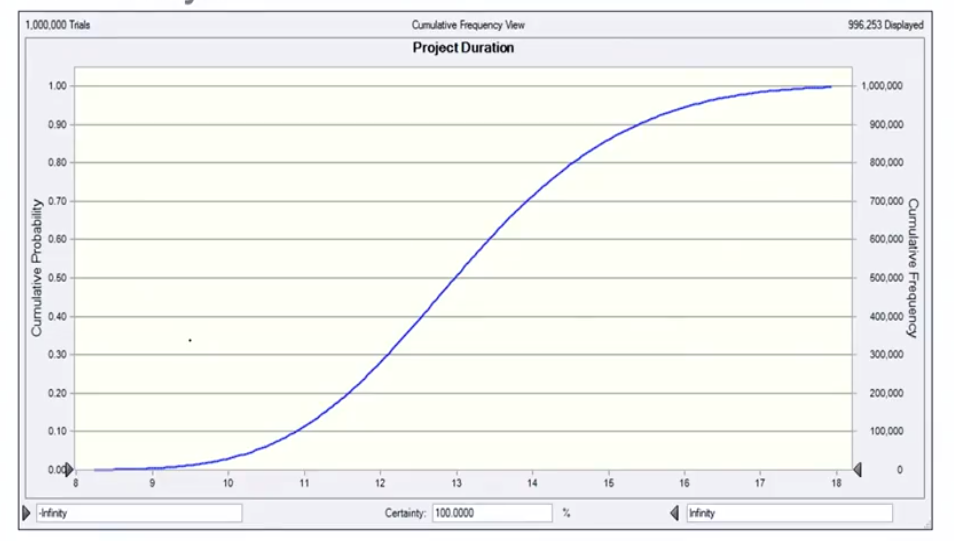
\includegraphics[width = 0.9\textwidth]{figs/fig13.png}
  \end{figure}
\end{frame}

\begin{frame}
 \frametitle{Roadmap no lugar de plano}
  \begin{figure}
   \centering
   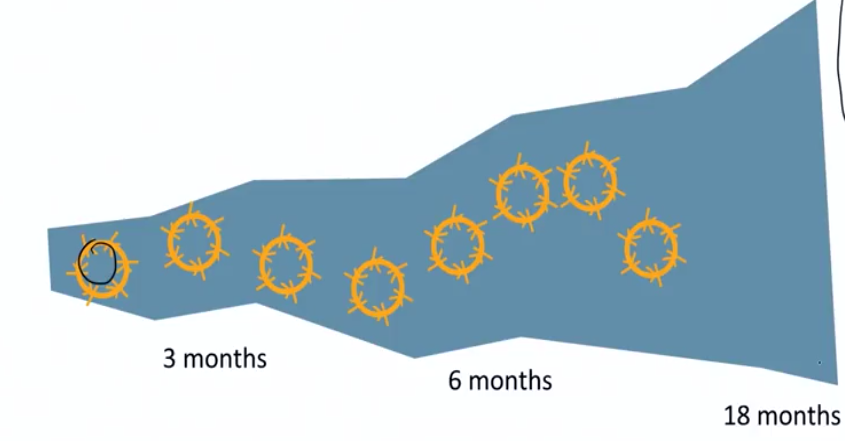
\includegraphics[width = 0.9\textwidth]{figs/fig14.png}
  \end{figure}
\end{frame}

\begin{frame}
 \frametitle{Roadmap no lugar de plano}
  \begin{figure}
   \centering
   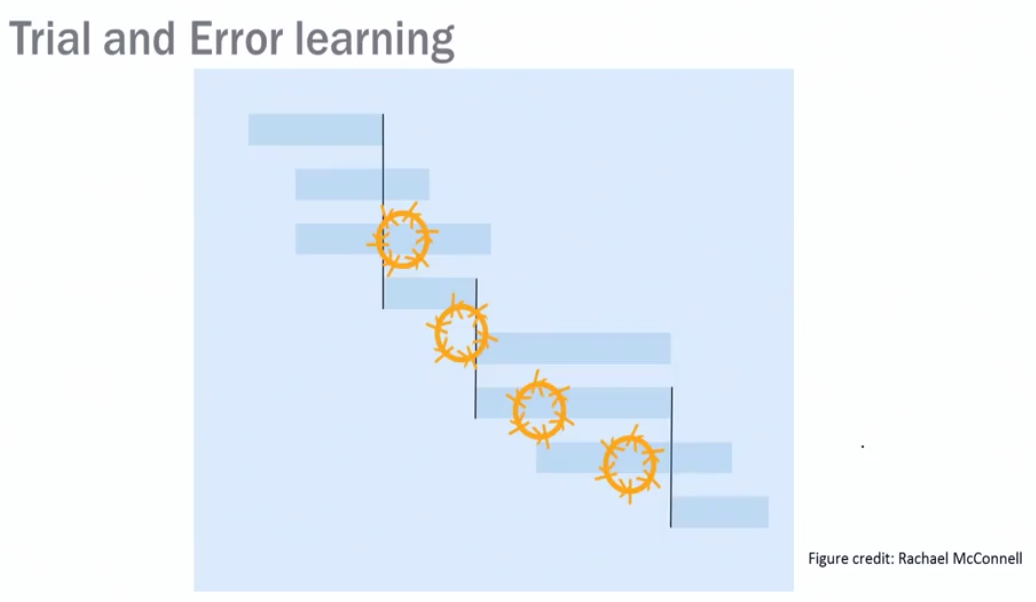
\includegraphics[width = 0.9\textwidth]{figs/fig15.png}
  \end{figure}
\end{frame}